\documentclass[a4paper,12pt]{article}
\usepackage[T2A]{fontenc}
\usepackage[cp1251]{inputenc}
\usepackage[english,russian]{babel}
\usepackage{amssymb,amsfonts,amsmath,cite,enumerate,float,indentfirst}
\usepackage{graphicx} 
\usepackage{float}
\usepackage{wrapfig}
\usepackage{array}
\usepackage{geometry}
\geometry{left=2cm}
\geometry{right=1.5cm}
\geometry{top=1cm}
\geometry{bottom=2cm}





\newcommand{\imgh}[3]
{
\begin{figure}[h]
\center{\includegraphics[width=#1]{#2}}
\caption{#3}
\label{ris:#2}
\end{figure}
}


\begin{document}
\begin{titlepage}
\newpage

\begin{center}
МИНОБРНАУКИ РОССИИ

Федеральное государственное автономное образовательное учреждение

высшего образования

\textbf{«Омский государственный университет им. Ф.М. Достоевского»} \\
\end{center}

\vspace{10em}



\begin{center}
\textsc{\textbf{Отчет \linebreak по учебной практике}}
\end{center}

\vspace{25em}



\newbox{\lbox}
\savebox{\lbox}{\hbox{Потапов Артем Витальевич}}
\newlength{\maxl}
\setlength{\maxl}{\wd\lbox}
\hfill\parbox{11cm}{
\hspace*{5cm}\hspace*{-5cm}Студент:\hfill\hbox to\maxl{Потапов Артем Витальевич\hfill}\\
\hspace*{5cm}\hspace*{-5cm}Преподаватель:\hfill\hbox to\maxl{Богаченко Надежда Федоровна}\\
\\
\hspace*{5cm}\hspace*{-5cm}Группа:\hfill\hbox to\maxl{МПБ-101-0-01}\\
}


\vspace{\fill}

\begin{center}
Омск \\2023
\end{center}

\end{titlepage} 

\newpage
\tableofcontents 
\newpage

\part {Введение}

Целями учебной практики являются закрепление, расширение и
углубление полученных во время выполнения проекта теоретических знаний, а
также приобретения первоначальных практических умений в выбранной
студентом сфере. В своей работе я планирую научиться работать с реальным
игровым движком и создать собственную игру
\newline
Перед собой я ставил цель ознакомиться со средствами, используемыми
для создание игры на игровом движке Unity, а также с особенностью написания
скриптов для видеоигр.
\newline
На учебной практике я поставил перед собой следующие задачи:
\newline
\begin{itemize}
\item  Изучение материалов, необходимых для разработки видеоигры а
также языка C шарп.
\item  Разбиение разработки на несколько этапов создания механик.
\item  Написание скриптов и расстановка моделей в Unity 3D.
\end{itemize}
Моей целью на первый семестр является написание скриптов для передвижения
персонажа и NPC, взаимодействие игрока с врагами, а также разработка
основных механик инвентаря.
\newpage
\section {Глава 1 Изучение материалов}
\subsection{ Изучение языка программирования C Шарп.}
Так как создание игры и написание скриптов на игровом движке Unity
происходит на языке программирования C Шарп, то я решил начать создавать свой
проект с изучения этого языка. У меня уже был опыт написания различных
программ на других языках, таких как C++ и Python, а значит изучать основы
программирования мне не требовалось. Я решил изучать C Шарп через видеоуроки,
а точнее через видеохостинг YouTube. На данном сервисе огромное количество
видеоуроков, однако я остановился на канале SimpleCode, там мне следового я
с особенностями синтаксиса C Шарп, а также с его основными функциями. \newline
\subsection{ Изучение особенностей движка Unity}
Далее мне предстояло изучить самое главное, а именно работу с движком
Unity. В поиске материалов не было никаких проблем, так как вся информация
есть в официальной документации на сайте Unity. \newline
Начал я обучение с изучения инструментов для создания объектов и
работы со скриптами. После этого я начал переходить к основе. Я изучил
работу с многими методами классов, триггерами, работы с интерфейсом,
основы перемещения, физики и так далее. На это у меня ушло около полутора
месяцев.

\newpage
\section {Глава 2. Создание игры и написание скриптов}
\subsection{Изучение аналогов.}
Конечно для разработки видеоигры и ее основных механик я
ориентировался на проекты схожие с моим. В итоге я выбрал 5 проектов
наиболее схожим с моим, а именно: “ Dragon Age :Origins”, “ Harry Potter”,
“Mages of Mystralia”, “ Atom RPG”, “ Tales of Arise”
Таблица 1. Обзор аналогов \newline
\begin {center}
\begin{tabular}{ | m{6em} | m{3cm}| m{5cm} | m{3cm} | m{3cm} | } 
 \hline
Название & Движок & Цель & Управление & Жанр\\
 \hline
 Dragon Age:Origins &  ECLIPSE &путешествие
мага-воина с
целью
уничтожения
зла &мышь & фэнтези, вид
сверху, экшн,
RPG\\
\hline
 Harry Potter &Unreal Engine 4 &путешествие
ученика у
волшебной
школе с
целью
уничтожения
зла и
изучению
новых
заклинаний& мышь и
клавиатура&фэнтези, вид
сверху, экшн\\
\hline 
Mages of Mystralia & unity & победить
могучих
существ и
пройти
квесты, с
помощью
изучения
заклинаний & мышь &экшн, квест \\
\hline 
Atom RPG & unity & человечество
на грани  вымирания,
путешествие с
целью
выжить и
расследовани
я странностей &мышь и
клавиатура & пошаговое RPG \\	
\hline 
Tales of Arise & unreal engine 4 &поиск
потерянных
воспоминани
й, сражение с
врагами,
прохождение
сюжетного
квеста &мышь & фэнтези,
ролевая игра,
экшн, RPG\\
\end{tabular}
\end{center}
После изучения аналогов я выяснил, что лучше делать не свободную
камеру, а фиксированную, чтобы игрок не отвлекался на ее настройку, также
понял, что передвижение лучше сделать на клавиши на клавиатуре, атаки
сделать на правую кнопку мыши.
\subsection{Создание тестовой локации.}
Так работа над моделями и локации еще велась другими членами моей
команды, я решил сделать для себя тестовою локацию для разработки. Я сделал
платформу, чтобы персонажи не падали во время запуска игры, а также сделал
главного героя в виде кубика, чтобы реализовать на нем передвижение и атаку.
\subsection{Написание скриптов движения.}
Первый скрипт который я написал, это скрипт передвижения камеры, это
был самый простой скрипт, так как стоило просто изменять позицию камеры
при изменении позиции игрока соответственно.
Далее писался скрипт передвижения. В нем задавалась скорость и ссылка
на объект, после этого в зависимости от нажатой клавиши, персонаж
перемещался на координату X или Z на каждом кадре.
\newline
\begin{figure}[h]

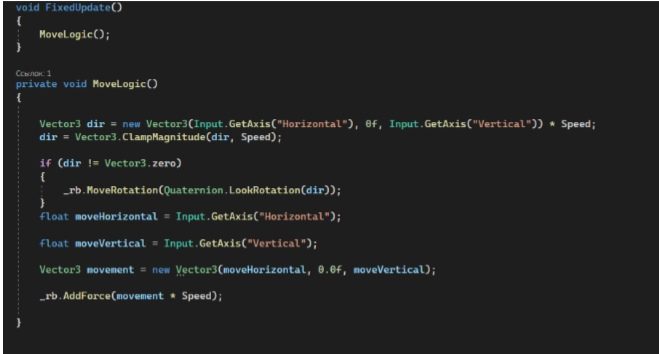
\includegraphics[width=0.8\linewidth]{forExample.jpg}

\caption{Скрипт, отвечающий за передвижение}

\label{fig:mpr}
\end{figure}
Дальше отчет идет в том же стиле
\newpage
\newpage
\newpage
\section{������ ����������}
\begin{itemize}
\item �������� �� �������� C���� URL:https://www.youtube.com/watch?v=KyFWqbRfWIAamp;list=PLQOaTSbfxUtD6kMmAYc8Fooqya3pjLs1N (���� ��������� 12.11.2022)
\item  ����������� ������������ Unity URL:https://docs.unity3d.com/Manual/
(���� ��������� 22.12.2022)
\item ���� �� ������� ���� ������ ������ �� ������� �� ��������� ����
https://ru.stackoverflow.com/ (���� ��������� 19.12.2022)
\item ����� ��� ���������� ������
https://www.youtube.com/watch?v=NyoEisCiN7A (���� ���������
2.11.2022)
\end{itemize}


\newpage
\end{document}